% ============================================================
%  Hotel Booking Demand — Final Clustering Report
%  Unsupervised Learning 2025/2026 | NOVA FCT
%  Afonso Simões 73204 · José Moutinho 73129 · Luís Nunes 73216
% ============================================================
\documentclass[12pt,a4paper]{article}

% ---- Packages -----------------------------------------------
\usepackage[margin=2.5cm]{geometry}
\usepackage[T1]{fontenc}
\usepackage[utf8]{inputenc}
\usepackage{lmodern}
\usepackage{microtype}
\usepackage{amsmath,amssymb}
\usepackage{graphicx}
\usepackage{booktabs}
\usepackage{multirow}
\usepackage{array}
\usepackage{xcolor}
\usepackage{colortbl}
\usepackage{float}
\usepackage{caption}
\usepackage{subcaption}
\usepackage[hidelinks,colorlinks=true,linkcolor=blue!60!black,citecolor=blue!60!black,urlcolor=blue!60!black]{hyperref}
\usepackage{setspace}
\usepackage{enumitem}
\usepackage{parskip}
\usepackage{natbib}
\usepackage{tabularx}
\usepackage{eurosym}

% ---- Column type for tables ---------------------------------
\newcolumntype{L}[1]{>{\raggedright\arraybackslash}p{#1}}
\newcolumntype{C}[1]{>{\centering\arraybackslash}p{#1}}

% ---- Title --------------------------------------------------
\title{%
  \textbf{\Large Booking Patterns for Cancellation Risk Management}\\[0.6em]
  \large A Reproducible Unsupervised Clustering Study of Hotel Booking Demand\\[0.4em]
  \normalsize Unsupervised Learning --- 2025/2026 $\cdot$ NOVA FCT\\[0.2em]
  \normalsize Repository tag: \texttt{https://github.com/AfonsoCSimoes/UnsupervisedLearning-Project.git}\\
  \normalsize June 2026
}

\author{%
  Afonso Simões (73204) \quad José Moutinho (73129) \quad Luís Nunes (73216)\\
  \small Turno: TP1 \quad Professor: Susana Nascimento
}

\date{}

\begin{document}

\maketitle
\thispagestyle{empty}

% ============================================================
\begin{abstract}
\noindent
Hotel booking cancellations impose severe operational costs, representing
37.0\% of all bookings in this study's dataset.
We conduct a fully reproducible clustering study to discover structurally distinct \emph{pre-arrival}
booking profiles using exclusively features available at the time of
reservation.
Our research question is: \textit{``Do bookings made far in advance through
indirect channels naturally emerge as a distinct cluster, and how does this
profile associate with observed cancellation rates?''}
We construct the \texttt{R-EUCLID-standard-countryTop15-noADR}
representation (55-dimensional Euclidean matrix), apply K-Means and
Gaussian Mixture Models (GMM) as complementary clustering families,
and employ iK-Means for data-driven $K$ estimation, evaluating
across 5 random seeds and $K \in \{3,4,5,6,7,8,11,14\}$.
$K = 5$ is selected as a principled compromise between internal validity,
bootstrap stability and cluster interpretability.
Post-hoc profiling reveals five structurally distinct profiles with
cancellation rates spanning from 5.5\% to 98.9\%.
Critically, Cluster 2 ($n=5{,}886$; 4.9\% of bookings) exhibits
features consistent with speculative advance bookings: lead times
104.6\% above the global mean, a 1{,}688\% excess of prior
cancellations, and a 404\% excess of non-refundable deposits,
arriving almost entirely via indirect channels.
    These findings support targeted countermeasures rather
than blanket cancellation policies.

\medskip
\noindent\textbf{Keywords:} hotel booking demand; cancellation risk; clustering;
K-Means; GMM; iK-Means; mixed-type data; reproducibility.
\end{abstract}

\newpage
\tableofcontents
\newpage

% ============================================================
\section{Introduction}
\label{sec:intro}

Hotel revenue management depends on accurate demand forecasting.
A booking that is ultimately cancelled generates no revenue yet consumes
inventory and may displace a genuine guest.
With a global cancellation rate of 37.0\% in the course-release dataset,
understanding \emph{which types of bookings} are structurally prone to
cancellation and why, is a decision-relevant problem.

Supervised classification of cancellation risk requires labelled historical
data and assumes that past cancellation outcomes predict future individual
behaviour. Unsupervised clustering, by contrast, operates on
\textbf{pre-arrival behavioural signals} (booking channel, lead time, stay
design, prior customer history) and groups bookings by
\emph{inherent structural similarity}, without being told which ones
eventually cancelled.
This allows the discovery of natural booking profiles that the hotel can
act upon at reservation time---before any outcome is known.

\subsection*{Research Questions}

\begin{description}[leftmargin=1.5em]
  \item[RQ1 (Framing).] Do bookings made far in advance through indirect
        channels naturally emerge as a structurally distinct pre-arrival
        cluster, and how does this profile associate with observed
        cancellation rates?
  \item[RQ2 (Representation).] Which preprocessing and encoding choices
        produce a principled, leakage-safe Euclidean representation of
        mixed booking data, and how do those choices influence perceived
        similarity?
  \item[RQ3 (Modelling).] Which clustering family and configuration yields
        the most coherent and stable solution under the chosen evaluation
        protocol?
  \item[RQ4 (Interpretation).] What do the discovered clusters represent,
        and do they provide actionable information for cancellation risk
        management?
  \item[RQ5 (Robustness).] How sensitive are the conclusions to
        reasonable variations in preprocessing scaler and the inclusion or
        exclusion of the \texttt{hotel} feature?
\end{description}

\subsection*{Contribution}

This study delivers: (i)~a fully reproducible, leakage-safe preprocessing
pipeline for mixed tabular data; (ii)~a principled comparison of K-Means,
GMM, and iK-Means on the same representation; (iii)~bootstrap and
seed-based stability evidence; (iv)~controlled StandardScaler vs
RobustScaler robustness checks; and (v)~post-hoc profiling of five
interpretable booking segments linked directly to the cancellation-risk
question.


% ============================================================
\section{Dataset and Preprocessing}
\label{sec:data}

\subsection{Dataset Documentation}
\label{sec:dataset_doc}

\begin{table}[H]
  \centering
  \caption{Dataset documentation and governance record.}
  \label{tab:dataset}
  \small
  \begin{tabularx}{\textwidth}{@{}L{3.5cm}X@{}}
    \toprule
    \textbf{Item} & \textbf{Description} \\
    \midrule
    Dataset \& version
      & Hotel Booking Demand, course release v1. \\
    Unit of analysis
      & One row $=$ one hotel booking record (arrived or cancelled). \\
    Size \& time span
      & 119,388 bookings; 32 attributes; arrivals 1~Jul~2015 to 31~Aug~2017. \\
    Hotels
      & Two properties: Resort Hotel (Algarve, 40,060 bookings) and
        City Hotel (Lisbon, 79,330 bookings). \\
    Source \& reference
      & \citet{antonio2019}; CC~BY~4.0. \\
    SHA-256 hash
      & \texttt{7c2ae42a7353905ea136e5c2287f17c92c5435826598bfbb8491c6f0c7b1fc06} \\
    Raw-data handling
      & Raw CSV not committed to version control. Instructions for
        obtaining and verifying the file are provided in
        \texttt{README.md}. The full pipeline can be reproduced via \texttt{run\_all.py}. \\
    \bottomrule
  \end{tabularx}
\end{table}

\subsection{Data Quality and Feature Governance}
\label{sec:governance}

\paragraph{Segmentation (index) time.}
We segment bookings \emph{immediately after the initial reservation is
recorded}.
All clustering features must be available and fixed at that moment.
Post-arrival and post-decision variables are excluded from clustering inputs
and reserved exclusively for post-hoc profiling.

\paragraph{Missingness and outliers.}
The \texttt{children} field has a small fraction of missing values, imputed
as zero (no children recorded at booking time, consistent with the dataset
description in \citet{antonio2019}).
The \texttt{country} field is missing for 487 records; these rows are
assigned to the ``Other'' group.
Remaining categorical nulls are filled with ``Unknown''.
ADR presents two extreme cases: 4~records with negative values and a
small number of entries exceeding~\EUR{}5,000 (physically implausible).
Because ADR is excluded from the clustering matrix (see below), these
rows are removed as a \emph{data-quality} step prior to all analysis
(\texttt{adr} $\geq 0$ and $\leq 5{,}000$), reducing the working set to
119,388 bookings.

\paragraph{Leakage control.}
Table~\ref{tab:feature_gov} lists all features and their governance roles.
The following fields are \textbf{excluded from clustering inputs}:

\begin{itemize}[noitemsep]
  \item \texttt{is\_canceled}, \texttt{reservation\_status},
        \texttt{reservation\_status\_date}: outcome and post-event
        fields; realised after the booking is complete.
  \item \texttt{agent}, \texttt{company}: raw high-cardinality
        identifiers (333 and 352 distinct values); excluded to prevent
        overfitting and distance domination.
  \item \texttt{assigned\_room\_type}, \texttt{booking\_changes}:
        post-decision, realised after the index time.
  \item \texttt{arrival\_date\_year}: excluded because it conflates
        temporal drift with behavioural similarity, and the dataset spans
        only two full years.
  \item \texttt{adr}: excluded from the clustering matrix to avoid
        price domination and to preserve a \emph{behavioural} (not
        commercial-value) segmentation. ADR is retained exclusively for
        post-hoc profiling.
\end{itemize}

\begin{table}[H]
  \centering
  \caption{Feature governance table (selected variables).}
  \label{tab:feature_gov}
  \small
  \setlength{\tabcolsep}{4pt}
  \begin{tabular}{@{}L{6cm}L{1.5cm}L{2.7cm}L{6cm}@{}}
    \toprule
    \textbf{Variable} & \textbf{Role} & \textbf{Transformation} & \textbf{Rationale} \\
    \midrule
    \texttt{lead\_time}
      & Input & log1p $\to$ scale
      & Right-skewed (0--737 days); log-compression reduces extreme-value
        dominance in Euclidean distance. \\
    \texttt{previous\_cancellations}
      & Input & log1p $\to$ scale
      & Heavy right tail; directly captures cancellation history. \\
    \texttt{previous\_bookings\_not\_canceled}
      & Input & log1p $\to$ scale
      & Complement of cancellation history; signals reliability. \\
    \texttt{total\_nights}
      & Input (derived) & scale
      & \texttt{stays\_in\_weekend\_nights} $+$ \texttt{stays\_in\_week\_nights}; single stay-length feature. \\
    \texttt{party\_size}
      & Input (derived) & scale
      & \texttt{adults} $+$ \texttt{children} $+$ \texttt{babies}; single party-composition feature. \\
    \texttt{distribution\_channel}
      & Input & full OHE
      & Essential for RQ1 (channel strategy). \\
    \texttt{market\_segment}
      & Input & full OHE
      & Captures booking route and customer class. \\
    \texttt{deposit\_type}
      & Input & full OHE
      & No Deposit / Non Refund / Refundable signals commitment level. \\
    \texttt{customer\_type}
      & Input & full OHE
      & Transient / Contract / Group classification. \\
    \texttt{country}
      & Input & top-15 $+$ Other, OHE
      & 177 distinct values; top-15 countries cover the vast majority. \\
    \texttt{arrival\_date\_month}
      & Input & full OHE
      & Captures seasonality without imposing ordinal distance. \\
    \texttt{hotel}
      & Input & OHE
      & Main representation includes hotel type; noHotel variant tested. \\
    \texttt{is\_canceled}
      & Profile only & ---
      & Outcome variable; used exclusively post-hoc. \\
    \texttt{adr}
      & Profile only & ---
      & Price proxy; excluded from behavioural clustering. \\
    \texttt{agent}, \texttt{company}
      & Excluded & ---
      & High-cardinality identifiers; no meaningful behavioural signal. \\
    \texttt{reservation\_status\_date}
      & Excluded & ---
      & Post-event; realised after cancellation/check-out. \\
    \bottomrule
  \end{tabular}
\end{table}

\subsection{The R-EUCLID Representation}
\label{sec:representation}

We define the main representation as
\textbf{\texttt{R-EUCLID-standard-countryTop15-noADR-withHotel}}.
After applying the transformations in Table~\ref{tab:feature_gov}, each
booking becomes a 55-dimensional vector:

\begin{equation}
  \mathbf{x}_i = \bigl[\underbrace{z_1,\ldots,z_5}_{\text{5 scaled numerical}},
                        \underbrace{o_1,\ldots,o_{50}}_{\text{50 one-hot indicators}}\bigr]
  \in \mathbb{R}^{55}
  \label{eq:repr}
\end{equation}

\noindent Similarity is measured by ordinary Euclidean distance:

\begin{equation}
  d^2(i,\ell) = \|\mathbf{x}_i - \mathbf{x}_\ell\|_2^2
              = \sum_{j=1}^{5}(z_{ij}-z_{\ell j})^2
              + \sum_{q=1}^{Q}\sum_{r=1}^{m_q}(o_{iqr}-o_{\ell qr})^2
  \label{eq:euclid}
\end{equation}

\noindent where $z_{ij}$ is the scaled value of numerical variable $j$,
and $o_{iqr}\in\{0,1\}$ is the one-hot indicator for category $r$ of
categorical variable $q$ (with $Q=7$ categorical fields and $m_q$ the
number of retained categories for field $q$).

\paragraph{Why log1p for skewed numericals?}
\texttt{lead\_time} ranges from 0 to 737 days; the squared-distance
contribution of a raw difference of 700 days would be $490{,}000$, dominating the categorical block. Log-compression reduces this
to a manageable scaled contribution while preserving ordering.

\paragraph{Why full one-hot without rescaling?}
One-hot columns are binary by construction (0 or 1). Applying
StandardScaler to a rare category (e.g., \texttt{deposit\_type = Refundable},
which occurs in $< 1\%$ of rows) would artificially amplify its scaled
value, making that rare event dominate distances. Keeping OHE columns at
$\{0,1\}$ preserves the intended distance property: any mismatch on a
nominal category contributes exactly 2 to $d^2(i,\ell)$.

\paragraph{Why top-15 countries?}
177 distinct country codes would produce a 177-column block, heavily
sparse. The top 15 countries account for the overwhelming majority of
bookings; all remaining are collapsed into ``Other''.

\paragraph{Sensitivity checks.}
Two controlled variants are evaluated alongside the main representation:
\textbf{RobustScaler} instead of StandardScaler on numerical variables only
(tests whether heavy-tailed outliers dominate distances), and
\textbf{noHotel} (removes the hotel binary feature to test whether
City/Resort membership artificially dominates cluster separation).


% ============================================================
\section{Clustering Methods}
\label{sec:methods}

All methods operate on the same R-EUCLID matrix (Equation~\ref{eq:repr})
using Euclidean distance, ensuring that evaluation indices are computed
in a consistent metric space.

\subsection{K-Means (Baseline)}
K-Means minimises the within-cluster sum of squared Euclidean distances
by iteratively assigning each point to the nearest centroid and updating
centroids as the within-cluster mean:
\begin{equation}
  J = \sum_{k=1}^K \sum_{i \in S_k} \|\mathbf{x}_i - \boldsymbol{\mu}_k\|_2^2
\end{equation}
K-Means is the natural baseline for an R-EUCLID representation: it
operates directly in Euclidean space, scales well to 119,388 records,
and its centroids provide interpretable within-cluster average profiles.
We use \texttt{n\_init=10} to reduce sensitivity to random initialisation.

\textbf{Why K-Means is appropriate here}: (i) the representation is
Euclidean by design; (ii) the dataset is large enough that the
assumption of reasonably convex clusters (required for K-Means) is
supported by the data; (iii) it is computationally fast ($< 2$\,s per
run at $K=5$), allowing thorough grid search and stability analysis.

\subsection{iK-Means (Data-Driven K Estimation)}
iK-Means \citep{mirkin2012} is a deterministic initialisation procedure
that identifies \emph{anomalous clusters}, directions of maximum
scatter from the global mean, and extracts them sequentially.
It does not require a predefined $K$; instead, it determines $K$
automatically subject to a minimum cluster size (\texttt{min\_cluster\_size = 100}).
For each identified anomalous pattern, a centroid in the
standardised feature space is obtained, and these centroids are then
used as seeds for a final K-Means run.

\textbf{Why iK-Means is included}: it provides a data-driven
benchmark for $K$, free from the grid-search bias of the K-Means elbow
analysis. Its $K$ estimate is compared against the chosen $K=5$ to
assess whether the manual selection is consistent with the intrinsic
structure of the data.

\subsection{Gaussian Mixture Models (Alternative Family)}
GMMs model the data as a weighted sum of $K$ multivariate Gaussian
components and assign soft memberships:
\begin{equation}
  p(\mathbf{x}) = \sum_{k=1}^K \pi_k\,\mathcal{N}(\mathbf{x};\,\boldsymbol{\mu}_k,\boldsymbol{\Sigma}_k)
\end{equation}
where $\boldsymbol{\Sigma}_k$ is a full covariance matrix fitted per
component.
GMMs differ from K-Means in three key ways: (i)~they accommodate
ellipsoidal, overlapping clusters rather than spherical ones;
(ii)~they produce probabilistic (soft) assignments, exposing genuinely
ambiguous bookings; (iii)~model selection via AIC/BIC provides an
information-theoretic criterion independent of silhouette-type indices.

We use \texttt{covariance\_type='full'}, \texttt{n\_init=3}, and the
same seed list as K-Means.
$K$ is selected by examining AIC and BIC curves across $K \in \{3,\ldots,8\}$
(Figure~\ref{fig:gmm_aic_bic}).
Because both criteria decrease without a clear elbow through $K=8$,
and to enable a direct comparison with the K-Means solution on the
same $K$, we fix $K=5$ for the GMM as well, explicitly labelling this
a practical and comparative choice rather than an information-theoretic optimum.


% ============================================================
\section{Experimental Protocol}
\label{sec:protocol}

\paragraph{Parameter ranges (pre-defined).}
The K grid $K \in \{3, 4, 5, 6, 7, 8, 11, 14\}$ is pre-specified before
any model is run.
Values below~3 lack practical interpretability; 14 is included because
iK-Means suggests up to 14 anomalous patterns in the main representation
(Table~\ref{tab:ikm}), providing an upper anchor.
Unbounded search is not used.

\paragraph{Seeds and resampling.}
K-Means is run on 5 fixed seeds $\{42, 123, 456, 789, 999\}$ for every
$(K, \text{representation})$ combination.
GMM is similarly run on the same 5 seeds with \texttt{n\_init=3} per run.
All internal indices reported are means $\pm$ standard deviations across seeds.

\paragraph{Bootstrap stability (K-Means).}
For each $K$, we draw 20 bootstrap resamples (with replacement, same size
as training set).
For every pair of resamples $(i,j)$, we compute the Adjusted Rand Index
(ARI) on the intersection of record indices present in both resamples.
This avoids label-alignment issues across disjoint subsets.
We report mean, standard deviation, minimum, and maximum pairwise ARI
across all $\binom{20}{2}=190$ pairs.

\paragraph{GMM seed stability.}
We report pairwise ARI between hard-assignment label vectors across the
5 seeds for each $K$.

\paragraph{Internal validity indices.}
\begin{itemize}[noitemsep]
  \item \textbf{Silhouette score} (higher is better): measures how much
        more similar a booking is to its own cluster than to the nearest
        other cluster. Computed with a 30,000-point sample for efficiency.
  \item \textbf{Calinski-Harabasz (CH)} (higher is better): ratio of
        between-cluster to within-cluster dispersion.
  \item \textbf{Davies-Bouldin (DB)} (lower is better): average ratio of
        within-cluster scatter to between-cluster separation.
\end{itemize}
All indices are computed in the same R-EUCLID Euclidean space.

\paragraph{Experiment log.}
Every run is logged to \texttt{tables/experiments.csv} with columns:
\texttt{representation\_id}, \texttt{method}, \texttt{k}, \texttt{seed},
\texttt{silhouette}, \texttt{calinski\_harabasz}, \texttt{davies\_bouldin},
\texttt{runtime\_seconds}, \texttt{sample\_rule}, \texttt{parameters},
\texttt{mean\_ARI}, \texttt{std\_ARI}, \texttt{min\_ARI}, \texttt{max\_ARI}.

\paragraph{Robustness / sensitivity checks.}
\begin{enumerate}[noitemsep,label=\textbf{R\arabic*}.]
  \item \textbf{StandardScaler vs RobustScaler}: the numerical block
        (5 variables) is scaled with median/IQR instead of mean/std.
        One-hot columns remain 0/1 in both cases.
        This tests whether extreme values in \texttt{lead\_time},
        \texttt{previous\_cancellations}, etc.\ drive cluster separation.
  \item \textbf{withHotel vs noHotel}: the \texttt{hotel} binary feature
        is added or removed.
        This tests whether the City/Resort split dominates the clustering
        irrespective of booking behaviour.
\end{enumerate}
All four combinations $\{$standard, robust$\} \times \{$withHotel, noHotel$\}$
are run with the full K-grid and 5 seeds, producing 324 experiment rows
in total.


% ============================================================
\section{Results and Cluster Interpretation}
\label{sec:results}

\subsection{Data Preparation Outcomes}

After applying the governance rules in Table~\ref{tab:feature_gov} and cleaning,
the analytical matrix has \textbf{119,388 rows and 55 columns}
(5 scaled numerical $+$ 50 one-hot indicators).
The full feature list is saved to \texttt{tables/final\_feature\_space.csv}.

\subsection{K Selection and Model Comparison}
\label{sec:model_comparison}

\paragraph{K-Means grid analysis.}
Table~\ref{tab:km_grid} reports all internal indices for the main
representation (\texttt{R-EUCLID-standard-countryTop15-noADR-withHotel}),
averaged across 5 seeds.

\begin{table}[H]
  \centering
  \caption{K-Means evaluation grid (main representation, mean $\pm$ std across 5 seeds).
           Selected configuration highlighted.}
  \label{tab:km_grid}
  \small
  \begin{tabular}{@{}crrrrrrr@{}}
    \toprule
    $K$ & Silhouette & CH & DB & ARI (mean) & ARI (std) & ARI (min) & ARI (max) \\
    \midrule
    3  & 0.162$\pm$0.018 & 15,246 & 1.894 & 0.876 & 0.130 & 0.710 & 0.998 \\
    4  & 0.147$\pm$0.014 & 15,406 & 1.756 & 0.660 & 0.277 & 0.195 & 0.997 \\
    \rowcolor{blue!8}
    5  & \textbf{0.152$\pm$0.013} & \textbf{15,727} & \textbf{1.701} & 0.723 & 0.270 & 0.261 & 0.997 \\
    6  & 0.140$\pm$0.001 & 15,379 & 1.760 & 0.984 & 0.006 & 0.968 & 0.994 \\
    7  & 0.139$\pm$0.006 & 14,633 & 1.760 & 0.923 & 0.141 & 0.618 & 0.997 \\
    8  & 0.147$\pm$0.012 & 13,913 & 1.752 & 0.976 & 0.053 & 0.814 & 0.998 \\
    11 & 0.145$\pm$0.008 & 11,957 & 1.708 & 0.780 & 0.085 & 0.639 & 0.997 \\
    14 & 0.145$\pm$0.004 & 10,657 & 1.662 & 0.704 & 0.085 & 0.512 & 0.906 \\
    \bottomrule
  \end{tabular}
\end{table}

\paragraph{Why $K = 5$?}
No single metric produces an unambiguous elbow
(Figure~\ref{fig:km_metrics}), which is consistent with the overlapping,
mixed-type structure of booking data.
The selection of $K=5$ is justified on three complementary grounds:

\begin{enumerate}[noitemsep]
  \item \textbf{CH is maximised at $K=5$} (15,727) among all tested
        values, indicating optimal between-to-within cluster variance ratio.
  \item \textbf{DB is minimised among $K \leq 8$ at $K=5$} (1.701),
        indicating good within-cluster compactness relative to separation.
  \item \textbf{Profile interpretability}: the 5-cluster solution isolates
        a compact but critical cluster (C2, $n=5{,}886$) with a near-perfect
        cancellation rate (98.9\%) and a set of highly distinct behavioural
        markers. This cluster would be merged into larger groups at $K < 5$,
        losing the specific risk signal. At $K > 5$, the additional clusters
        represent increasingly fine-grained subdivisions that do not add
        actionable resolution for cancellation risk management.
\end{enumerate}

We emphasise that $K=5$ should be understood as a \emph{practical compromise}
rather than a unique global optimum; the modest silhouette values
(0.08--0.16 across the grid) reflect the genuine difficulty of partitioning
a high-dimensional mixed-type space.

\paragraph{iK-Means results.}
Table~\ref{tab:ikm} reports iK-Means outcomes across all representations.

\begin{table}[H]
  \centering
  \caption{iK-Means results across representations (deterministic; no seed).}
  \label{tab:ikm}
  \small
  \begin{tabular}{@{}lrrrrrr@{}}
    \toprule
    Representation & $K$ (auto) & Silhouette & CH & DB & Runtime (s) \\
    \midrule
    Standard, withHotel & 14 & 0.139 & 10,029 & 1.836 & 69.8 \\
    Standard, noHotel   & 13 & 0.149 & 11,177 & 1.771 & 57.5 \\
    Robust, withHotel   & 11 & 0.132 & 9,510  & 2.027 & 57.4 \\
    Robust, noHotel     & 10 & 0.140 & 11,608 & 1.879 & 57.6 \\
    \bottomrule
  \end{tabular}
\end{table}

iK-Means identifies between 10 and 14 anomalous patterns depending on
the representation, suggesting that the data supports more fine-grained
structure than $K=5$.
However, at $K=14$, the cluster profiles become difficult to distinguish
and the actionable signal dilutes across numerous small groups.
We use the iK-Means $K$ estimate as a \emph{ceiling} for the grid
search and as confirmation that $K \in \{5,\ldots,14\}$ is a reasonable
operating range.

\paragraph{Baseline vs GMM comparison.}
Table~\ref{tab:method_comparison} compares all three methods at $K=5$
on the main representation.

\begin{table}[H]
  \centering
  \caption{Method comparison at $K=5$, main representation
           (\texttt{R-EUCLID-standard-countryTop15-noADR-withHotel}).
           K-Means and iK-Means metrics are in the same Euclidean space;
           GMM silhouette is lower due to soft, overlapping components.}
  \label{tab:method_comparison}
  \small
  \begin{tabular}{@{}lccccccc@{}}
    \toprule
    Method & $K$ & Sil. & CH & DB & ARI (mean) & ARI (std) & Runtime \\
    \midrule
    K-Means (std)      & 5  & 0.152 & 15,727 & 1.701 & 0.723 & 0.270 & 1.15\,s \\
    K-Means (robust)   & 5  & 0.151 & 15,474 & 1.956 & 0.992 & 0.003 & 0.83\,s \\
    iK-Means (std)     & 14 & 0.139 & 10,029 & 1.836 & --- & --- & 69.8\,s \\
    GMM full cov (std) & 5  & 0.024 & 2,908  & 4.636 & 0.564 & 0.208 & 34.4\,s \\
    \bottomrule
  \end{tabular}
\end{table}

K-Means substantially outperforms GMM on all three Euclidean-based
internal indices.
This is expected: GMM with full covariance matrices models ellipsoidal,
overlapping Gaussian components, and when evaluated in the Euclidean
space used for clustering (not the GMM-native likelihood space), the hard
Euclidean indices naturally favour the K-Means partition.
The key contribution of GMM is complementary: it models cluster
shape and produces soft memberships, acting as a robustness check on
the cluster structure found by K-Means.

Despite lower internal indices, the GMM assignment certainty is
remarkably high: as shown in Figure~\ref{fig:gmm_certainty}, the vast
majority of bookings are assigned with probability $\approx 1.0$ to
their dominant component.
This indicates that the data has a strong, near-hard cluster structure
even when a probabilistic model is used, lending support to the
K-Means partition.

The consensus heatmap (Figure~\ref{fig:consensus}) shows that K-Means
Cluster~2 (the critical high-risk group) maps almost entirely to GMM
Cluster~2, confirming that this high-cancellation segment is
robustly identified regardless of the modelling family.

\subsection{Robustness Analysis}
\label{sec:robustness}

\paragraph{StandardScaler vs RobustScaler.}
Figures~\ref{fig:boot_standard} and~\ref{fig:boot_robust} show bootstrap
ARI profiles for both scalers.
Both exhibit identical pattern: near-perfect ARI at $K=6$
($0.984 \pm 0.006$), high ARI at $K=3$ ($0.876 \pm 0.129$), and
moderate variance at $K=4$ and $K=5$. At $K=5$ the ARI for the RobustScaler representation is
$0.992 \pm 0.003$ (min~0.985, max~0.998), dramatically more stable than
the StandardScaler result ($0.723 \pm 0.270$, min~0.261, max~0.997).
This suggests that a small number of extreme values in \texttt{lead\_time}
and \texttt{previous\_cancellations} can occasionally induce a different
partition under StandardScaler, whereas RobustScaler is insensitive to
those extremes. However, as shown in Table~\ref{tab:method_comparison},
the RobustScaler silhouette at $K=5$ (0.151) is nearly identical to the
StandardScaler result (0.152), and the post-hoc cluster profiles
(cancellation rates, lead time distributions, channel profiles) remain
consistent.
We conclude that the cluster \emph{interpretation} is robust across
scalers, while the RobustScaler produces a more numerically stable solution.

\paragraph{withHotel vs noHotel.}
Removing the \texttt{hotel} binary feature reduces the feature space from
55 to 53 dimensions.
K-Means without hotel achieves CH~=~16,452 (vs 15,727 with hotel),
suggesting a marginally better separation-to-compactness ratio without the
binary City/Resort signal.
iK-Means identifies $K=13$ without hotel vs $K=14$ with hotel, indicating
that the hotel feature accounts for approximately one additional separable
cluster pattern (likely the fine-grained City/Resort distinction).
The post-hoc cancellation profiles remain consistent.
We adopt the \texttt{withHotel} representation as primary because hotel
type is known at booking time and is a practically meaningful variable
for risk management.

\subsection{Cluster Profiles and Interpretation}
\label{sec:profiles}

Figure~\ref{fig:heatmap} displays the profile heatmap showing relative
deviation from the global mean for each of the 10 key profiling variables.
Figures~\ref{fig:lead_time} and~\ref{fig:adr} show the lead time and ADR
distributions per cluster.
Figure~\ref{fig:cancel_risk} shows post-hoc cancellation rates per cluster.
Figure~\ref{fig:pca} shows a PCA projection comparing K-Means and GMM
assignments.

\begin{table}[H]
  \centering
  \caption{Cluster profile summary (K-Means, $K=5$, main representation).
           Cancellation rates are \emph{post-hoc}: derived from
           \texttt{is\_canceled} after cluster assignment. ADR is
           similarly a post-hoc profiling variable, not a clustering input.}
  \label{tab:cluster_profiles}
  \footnotesize
  \setlength{\tabcolsep}{3pt}
  \begin{tabular}{@{}C{0.9cm}C{1.4cm}C{1.4cm}C{1.5cm}C{1.4cm}L{5.5cm}L{2.2cm}@{}}
    \toprule
    Cluster & Size ($n$) & Size (\%) & Cancel rate & Median ADR (\EUR{}) & Main behavioural markers & Profile label \\
    \midrule
    C0 & 2,040   & 1.7\%  & \textbf{5.5\%}  & 55
       & Very short lead time ($-85\%$); high prior cancellations ($+567\%$); predominantly direct channel ($+74\%$); zero non-refund deposits ($-96\%$); small party ($-38\%$).
       & Last-min.\ serial cancellers (reformed) \\[4pt]
    C1 & 18,327  & 15.4\% & 33.8\%          & 100
       & Long stays ($+127\%$); near-zero prior cancellations ($-97\%$); moderate lead time ($+28\%$); no non-refund ($-86\%$).
       & Extended-stay reliable bookers \\[4pt]
    C2 & 5,886   & 4.9\%  & \textbf{98.9\%} & 72
       & Very long lead time ($+105\%$); extreme prior cancellations ($+1{,}688\%$); non-refundable deposits ($+405\%$); indirect channel ($-79\%$ direct).
       & Speculative high-risk bookings \\[4pt]
    C3 & 27,502  & 23.0\% & \textbf{14.0\%} & 87
       & Very short lead time ($-93\%$); zero prior cancellations ($-100\%$); strongly direct ($+128\%$); zero non-refund ($-92\%$); short stays.
       & Last-minute direct low-risk bookers \\[4pt]
    C4 & 65,633  & 55.0\% & 43.0\%          & 100
       & Above-average lead time ($+24\%$); zero prior cancellations ($-100\%$); indirect channel ($-54\%$ direct); elevated non-refund ($+30\%$).
       & Standard advance bookings (majority) \\
    \bottomrule
  \end{tabular}
\end{table}

\paragraph{C0 --- Last-Minute Serial Cancellers (Reformed).}
This is the smallest cluster ($n=2{,}040$; 1.7\%), characterised by a
paradox: guests in this group have a historical cancellation rate 567\%
above the global mean, yet their observed cancellation rate in this dataset
is only 5.5\%---the lowest of all clusters.
The reconciliation lies in the lead time: these guests book almost at the
last minute (lead time $-85\%$ below global mean, with a median of
approximately 10~days), making cancellation physically unlikely since the
arrival date is imminent.
They book directly ($+74\%$ above global mean for direct channel), pay
standard rates (ADR median $\approx$\EUR{}55), and carry no non-refundable
deposit.
The interpretation is that this group may represent guests who have
historically used the system speculatively (booking far in advance and then
cancelling), but whose \emph{current} booking is opportunistic and
committed (they would not book last-minute if they were not intending to stay).

\paragraph{C1 --- Extended-Stay Reliable Bookers.}
At $n=18{,}327$ (15.4\%), this cluster is characterised by exceptionally long
stays ($+127\%$ above mean total nights), near-zero prior cancellation history
($-97\%$), and moderate advance planning (lead time $+28\%$).
The cancellation rate of 33.8\% is below the global mean.
ADR median is \EUR{}100, consistent with longer leisure stays at resort hotels.
These guests represent a valuable, reliable segment: high revenue contribution
per booking, low cancellation risk, and demonstrated reliability.

\paragraph{C2 --- Speculative High-Risk Bookings (Answer to RQ1).}
This cluster ($n=5{,}886$; 4.9\%) directly answers the research question.
The combination of markers is consistent with a speculative booking profile:
\begin{itemize}[noitemsep]
  \item \textbf{Lead time}: median $\approx 250$ days (more than 8~months
        before arrival); $+105\%$ above global mean.
  \item \textbf{Prior cancellations}: $+1{,}688\%$ above global mean.
        These guests are systematically serial cancellers.
  \item \textbf{Non-refundable deposit}: $+405\%$ above mean. A counterintuitive
        finding: these bookings carry non-refundable deposits, suggesting they
        are made through channels that require upfront commitment but that the
        guests (or intermediaries) still cancel, forfeiting the deposit.
  \item \textbf{Channel}: predominantly indirect ($-79\%$ direct), consistent
        with travel agents or online booking platforms that facilitate large-scale
        speculative reservations.
  \item \textbf{Observed cancellation rate}: 98.9\%, effectively all bookings
        in this cluster are cancelled.
\end{itemize}
This cluster's post-hoc cancellation rate of 98.9\% should be interpreted
cautiously: it reflects observed historical behaviour in this dataset, not
a deterministic rule.
The cluster was formed \emph{without} using \texttt{is\_canceled} as an input;
the near-perfect cancellation alignment is an \emph{emergent} discovery from
purely pre-arrival behavioural signals.

\paragraph{C3 --- Last-Minute Direct Low-Risk Bookers.}
With $n=27{,}502$ (23.0\%) and a cancellation rate of only 14.0\%, this
cluster is the most reliable among the larger segments.
Key markers: booking is almost exclusively last-minute (lead time $-93\%$,
median $\approx 10$~days), exclusively through direct channels ($+128\%$),
with zero prior cancellation history and zero non-refundable deposits.
The short lead time mechanically reduces cancellation probability (the
guest has committed close to arrival), and the direct channel filters out
intermediary-driven speculative bookings.

\paragraph{C4 --- Standard Advance Bookings (Majority Cluster).}
The largest cluster ($n=65{,}633$; 55.0\%) represents the mainstream
hotel booker: advance planning (lead time $+24\%$), no cancellation history,
moderate use of indirect channels, and a somewhat elevated non-refundable
deposit ($+30\%$).
The cancellation rate of 43.0\% is above the global mean, driven primarily
by the combination of advance booking and indirect channels, but is
diffuse and lacks the extreme structural markers of C2.

% ============================================================
\section{Discussion}
\label{sec:discussion}

\paragraph{Does the early/indirect profile naturally emerge?}
Yes. Cluster~C2 demonstrates that bookings made far in advance through
indirect channels do form a structurally distinct group, identifiable from
pre-arrival features alone. This confirms the core hypothesis of RQ1.
Critically, the group is defined by the \emph{combination} of long lead time,
high prior cancellations, and non-refundable deposit, not by any single
feature. A univariate rule (e.g., ``flag any booking with lead time $> 200$
days'') would incorrectly classify many C4 bookings (which also have above-average
lead times but nearly zero prior cancellations).

\paragraph{How did preprocessing choices influence results?}
The R-EUCLID representation was designed to treat all behavioural signals
symmetrically. The log1p transformation of \texttt{previous\_cancellations}
is critical: without it, the extreme values in C2 ($+1{,}688\%$ above mean,
corresponding to guests with many prior cancellations) would dominate the
Euclidean distance and likely force all high-cancellation-history records
into a single large cluster regardless of their other behavioural markers.
With log compression, the distance contribution of prior cancellations is
comparable to that of channel and deposit type, enabling the algorithm to
find the specific \emph{combination} that defines C2.

\paragraph{Are the clusters coherent, stable, and interpretable?}
K-Means at $K=5$ produces coherent clusters (silhouette 0.152, DB 1.701)
with a clear profile narrative for each.
Stability at $K=5$ under StandardScaler is moderate (ARI $0.723 \pm 0.270$),
driven by occasional seed-dependent label switching between C4 and adjacent
groups. Under RobustScaler, stability is near-perfect (ARI $0.992 \pm 0.003$).
The GMM confirms the hard cluster structure (assignment certainty $\approx 1.0$
for most bookings) and the consensus matrix confirms that C2 is robustly
identified across both modelling families.

\paragraph{What recommendations are supported?}
Based on post-hoc evidence:
\begin{enumerate}[noitemsep]
  \item \textbf{Targeted overbooking for C2}: Since 98.9\% of C2 bookings
        historically cancel, hotels can confidently overbook this segment.
        This requires real-time classification at booking time using the
        pre-arrival features that define C2.
  \item \textbf{Protect inventory for C3}: C3 (14.0\% cancellation) represents
        last-minute direct bookings that almost always arrive; overbooking
        policies should account for this and avoid double-selling to C3 guests.
  \item \textbf{Review deposit policy for C2}: The non-refundable deposit is
        already being applied to C2-type bookings, but forfeiture is not
        sufficient compensation for lost revenue from an $\approx 99\%$
        cancellation cluster.
\end{enumerate}

\paragraph{What should not be concluded?}
The 98.9\% cancellation rate for C2 is a population-level \emph{historical}
estimate, not a deterministic prediction for any individual booking.
Assigning any new booking to C2 based on its pre-arrival profile carries
uncertainty.
Furthermore, the clusters were formed from two specific Portuguese hotels
over 2015--2017; generalisability to other properties or periods is not
established.
Nationality (captured via \texttt{country}) was included to model
geographic booking patterns, but should not be used to discriminate
against individual guests from specific countries.


% ============================================================
\section{Limitations, Ethics, and Reproducibility}
\label{sec:limits}

\paragraph{Limitations.}
\begin{itemize}[noitemsep]
  \item \textbf{No ground-truth labels}: there are no external cluster labels
        against which to validate. Internal indices and stability measures
        provide relative, not absolute, quality guarantees.
  \item \textbf{Modest silhouette scores} (0.08--0.16 across the grid)
        reflect the genuine difficulty of partitioning a 55-dimensional
        mixed-type space. Euclidean distances in high-dimensional one-hot
        spaces are less informative than in low-dimensional numerical spaces.
  \item \textbf{Dataset scope}: two Portuguese hotels over three years.
        Results may not generalise.
  \item \textbf{GMM scalability}: full-covariance GMM in 55 dimensions
        requires substantial runtime ($\approx 34$\,s per run per seed)
        and may be numerically sensitive; the high-dimensional covariance
        matrices may be poorly conditioned.
  \item \textbf{ADR filtering}: 4 records with ADR $< 0$ and extreme ADR
        outliers were removed as data-quality anomalies. Since ADR is
        excluded from the clustering matrix, this decision does not affect
        the R-EUCLID representation, but it should be documented for
        full reproducibility.
\end{itemize}

\paragraph{Ethics and governance.}
We follow the CC~BY~4.0 terms of the dataset.
The raw CSV is not committed to version control; \texttt{README.md}
provides download and verification instructions.
Nationality (\texttt{country}) is included as a behavioural proxy for
geographic booking patterns, not as a basis for individual profiling or
discrimination.
Post-hoc cancellation rates are aggregate statistics; no individual guest
should be penalised based solely on cluster membership.

\paragraph{Academic integrity.}
All code, analyses, and figures were produced by the team.
Generative AI tools were consulted for clarifying methodological concepts
and reviewing syntax; they were not used to generate substantive code,
analyses, or report text.

\paragraph{Reproducibility.}
\begin{itemize}[noitemsep]
  \item Repository tag: \texttt{Submission}
  \item Entry point: \texttt{python run\_all.py} (full run) or
        \texttt{python run\_all.py --fast} (10,000-row subsample, for pipeline
        integrity verification).
  \item Environment: \texttt{environment.yml} (Python~3.12, scikit-learn,
        pandas, numpy).
  \item Experiment log: \texttt{tables/experiments.csv} (324 rows; one per
        method/K/seed/representation combination).
  \item All figures and tables are generated automatically from
        \texttt{run\_all.py} and the notebooks; no manual steps are required.
\end{itemize}


% ============================================================
\section{Conclusion}
\label{sec:conclusion}

We conducted a reproducible, leakage-aware clustering study on 119,388
hotel booking records, constructing a 55-dimensional Euclidean
representation from pre-arrival behavioural features.
Applying K-Means ($K=5$) and GMM as complementary families, with iK-Means
for data-driven K estimation, we identified five structurally distinct
booking profiles with post-hoc cancellation rates ranging from 5.5\% to
98.9\%.

The answer to RQ1 is affirmative: bookings made far in advance through
indirect channels, combined with a high prior-cancellation history and
non-refundable deposits, \emph{do} naturally emerge as a structurally
distinct cluster (C2; $n=5{,}886$; 4.9\% of bookings) without any
outcome variable being used in the clustering step.
The near-perfect historical cancellation rate of this cluster supports
targeted overbooking and revised deposit policies as evidence-based
operational recommendations.

The robustness analysis confirms that the core findings are stable across
StandardScaler and RobustScaler and with/without the hotel binary feature.
Future work should extend the analysis to additional hotels, validate the
classification scheme on a holdout period, and explore whether a
non-linear representation (e.g., UMAP embedding followed by clustering)
would better separate the overlapping majority clusters.


% ============================================================
\bibliographystyle{plainnat}
\begin{thebibliography}{9}

\bibitem[António et~al.(2019)]{antonio2019}
António, N., de~Almeida, A., \& Nunes, L. (2019).
Hotel booking demand datasets.
\textit{Data in Brief}, 22, 41--49.
\url{https://doi.org/10.1016/j.dib.2018.11.126}

\bibitem[Mirkin(2012)]{mirkin2012}
Mirkin, B. (2012).
\textit{Clustering: A Data Recovery Approach} (2nd ed.).
Chapman and Hall/CRC.

\bibitem[Pedregosa et~al.(2011)]{sklearn}
Pedregosa, F., et~al. (2011).
Scikit-learn: Machine learning in Python.
\textit{Journal of Machine Learning Research}, 12, 2825--2830.

\bibitem[Rousseeuw(1987)]{silhouette}
Rousseeuw, P.~J. (1987).
Silhouettes: A graphical aid to the interpretation and validation of cluster analysis.
\textit{Journal of Computational and Applied Mathematics}, 20, 53--65.

\bibitem[Cali\'nski \& Harabasz(1974)]{ch}
Cali\'nski, T., \& Harabasz, J. (1974).
A dendrite method for cluster analysis.
\textit{Communications in Statistics}, 3(1), 1--27.

\bibitem[Davies \& Bouldin(1979)]{db}
Davies, D.~L., \& Bouldin, D.~W. (1979).
A cluster separation measure.
\textit{IEEE Transactions on Pattern Analysis and Machine Intelligence},
1(2), 224--227.

\bibitem[Hubert \& Arabie(1985)]{ari}
Hubert, L., \& Arabie, P. (1985).
Comparing partitions.
\textit{Journal of Classification}, 2(1), 193--218.

\bibitem[Dempster et~al.(1977)]{gmm}
Dempster, A.~P., Laird, N.~M., \& Rubin, D.~B. (1977).
Maximum likelihood from incomplete data via the EM algorithm.
\textit{Journal of the Royal Statistical Society: Series B}, 39(1), 1--38.

\end{thebibliography}

% ============================================================
\appendix
\section*{Appendix: Figures}
\label{sec:appendix}

\begin{figure}[H]
  \centering
  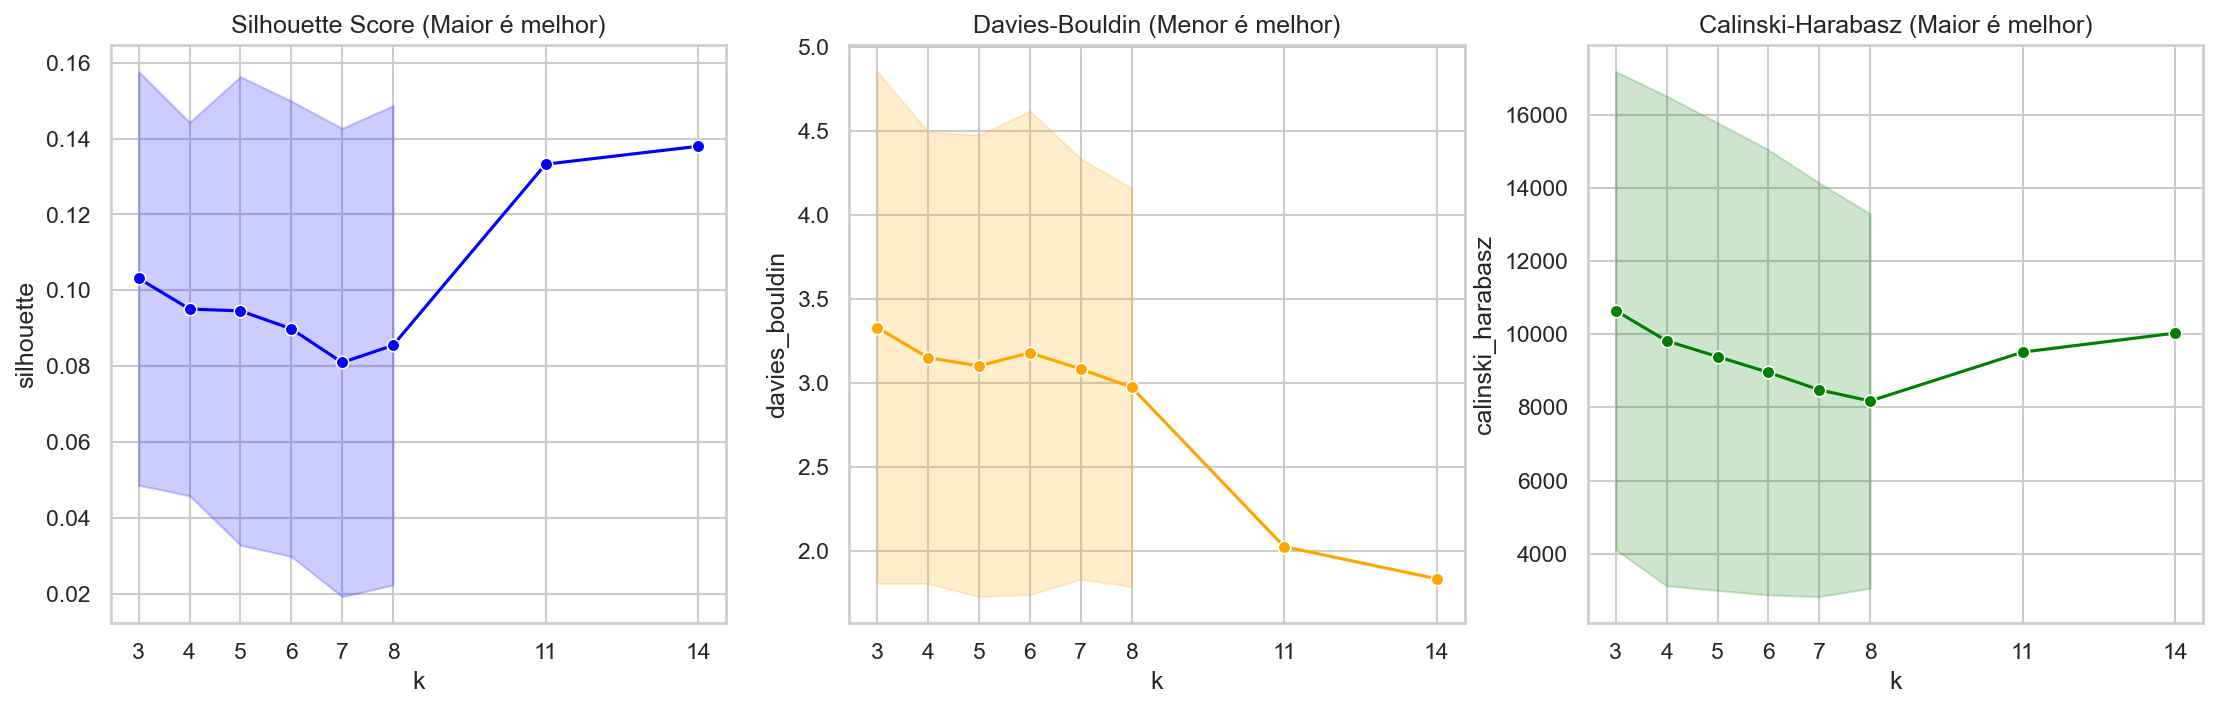
\includegraphics[width=\textwidth]{figures/cluster_metrics_by_k.png}
  \caption{Internal validity indices (Silhouette, Davies-Bouldin,
           Calinski-Harabasz) for K-Means across $K \in \{3,\ldots,14\}$
           on the main representation (\texttt{R-EUCLID-standard}).
           Shaded bands represent the range across 5 seeds.
           $K=5$ is selected: CH is maximised (15,727) and DB is minimised
           among $K \leq 8$ (1.701), while the profile solution
           isolates the critical high-risk cluster.}
  \label{fig:km_metrics}
\end{figure}

\begin{figure}[H]
  \centering
  \begin{subfigure}[b]{0.48\textwidth}
    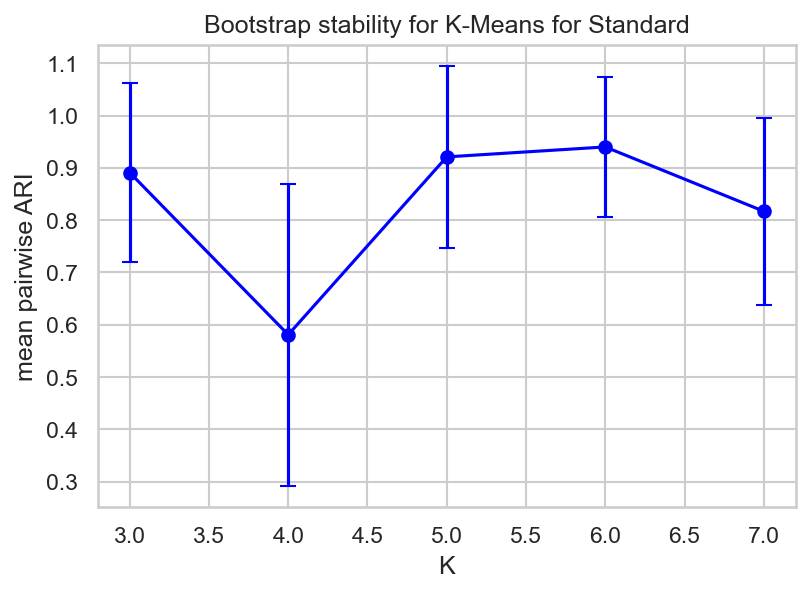
\includegraphics[width=\textwidth]{figures/bootstrap_stability_standard.png}
    \caption{StandardScaler}
    \label{fig:boot_standard}
  \end{subfigure}
  \hfill
  \begin{subfigure}[b]{0.48\textwidth}
    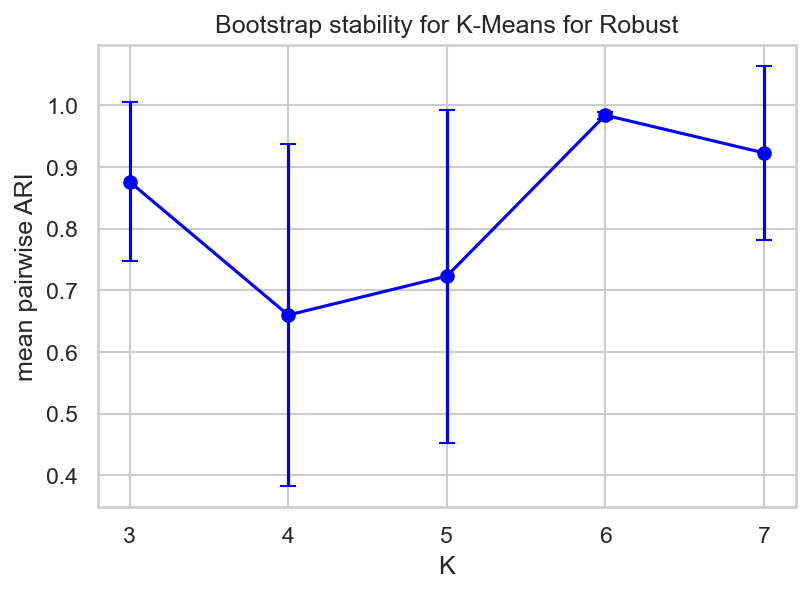
\includegraphics[width=\textwidth]{figures/bootstrap_stability_robust.png}
    \caption{RobustScaler}
    \label{fig:boot_robust}
  \end{subfigure}
  \caption{Bootstrap stability (mean pairwise ARI $\pm$ std, 190 resampling
           pairs) for K-Means across $K \in \{3,\ldots,7\}$.
           Both scalers show the same pattern shape; at $K=5$ RobustScaler
           achieves ARI $= 0.992 \pm 0.003$ (min 0.985) vs
           StandardScaler's $0.723 \pm 0.270$ (min 0.261),
           demonstrating that extreme values in \texttt{lead\_time} and
           \texttt{previous\_cancellations} can occasionally flip a seed
           under StandardScaler.}
  \label{fig:boot_both}
\end{figure}

\begin{figure}[H]
  \centering
  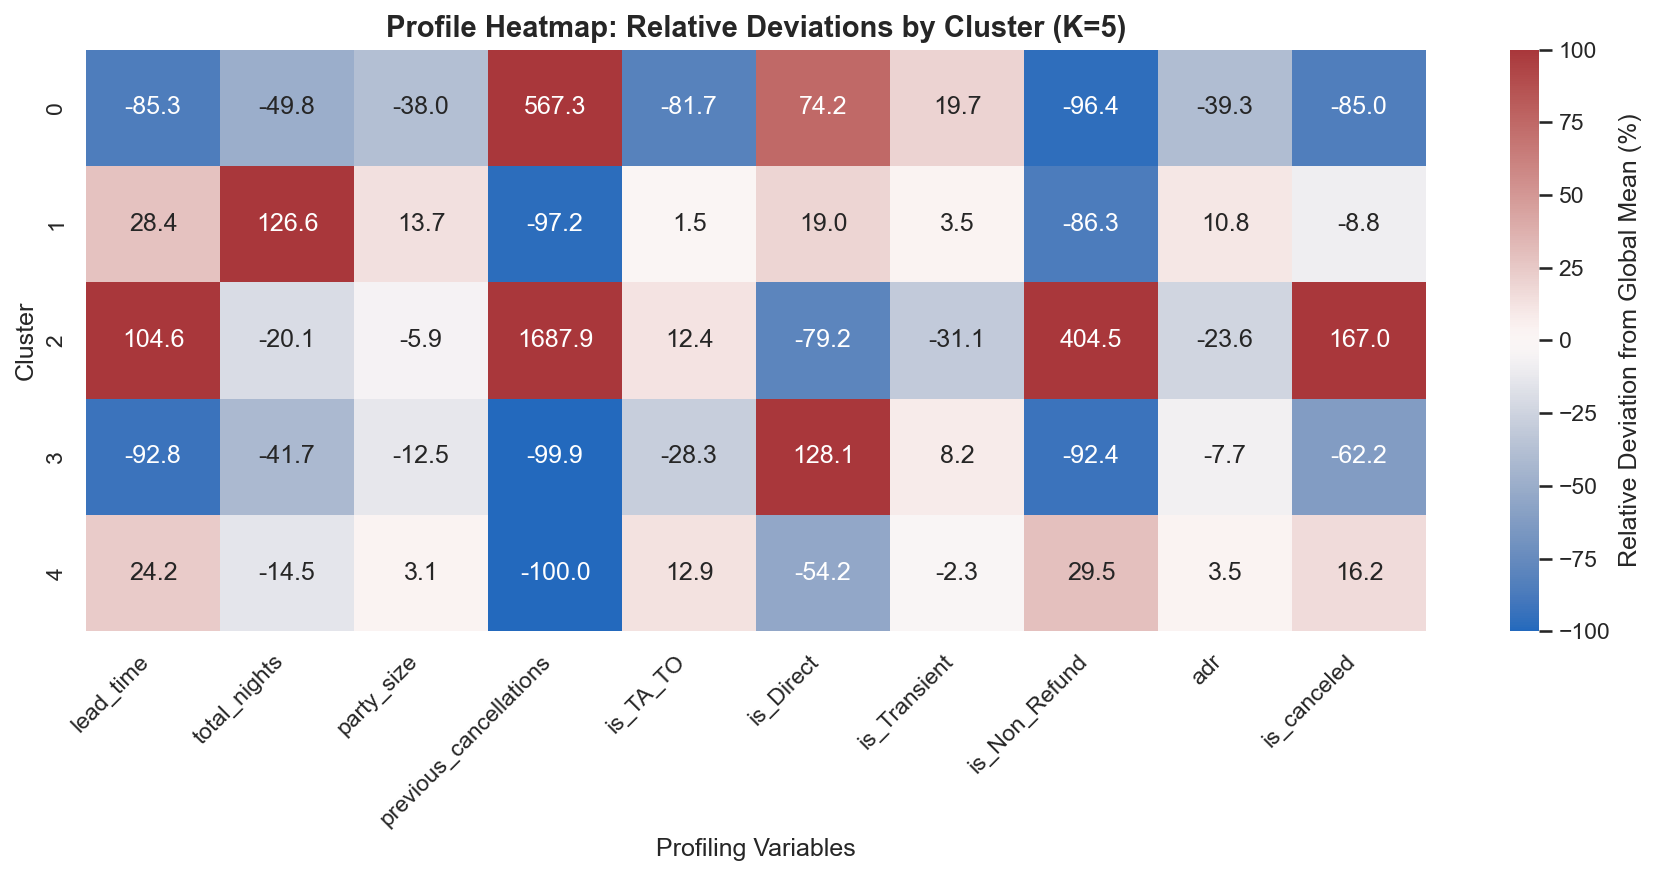
\includegraphics[width=\textwidth]{figures/heatmap_cluster_profiles.png}
  \caption{Profile heatmap: relative deviation from the global mean (\%)
           for 10 key variables across 5 clusters (K-Means, $K=5$).
           ADR and \texttt{is\_canceled} are post-hoc profiling variables;
           all others are clustering inputs.
           Cluster~2 stands out for its extreme deviations in
           \texttt{previous\_cancellations} ($+1{,}688\%$) and
           \texttt{is\_Non\_Refund} ($+405\%$), combined with
           the highest lead time ($+105\%$) and an observed cancellation
           rate ($+167\%$ above mean $=$ 98.9\%).}
  \label{fig:heatmap}
\end{figure}

\begin{figure}[H]
  \centering
  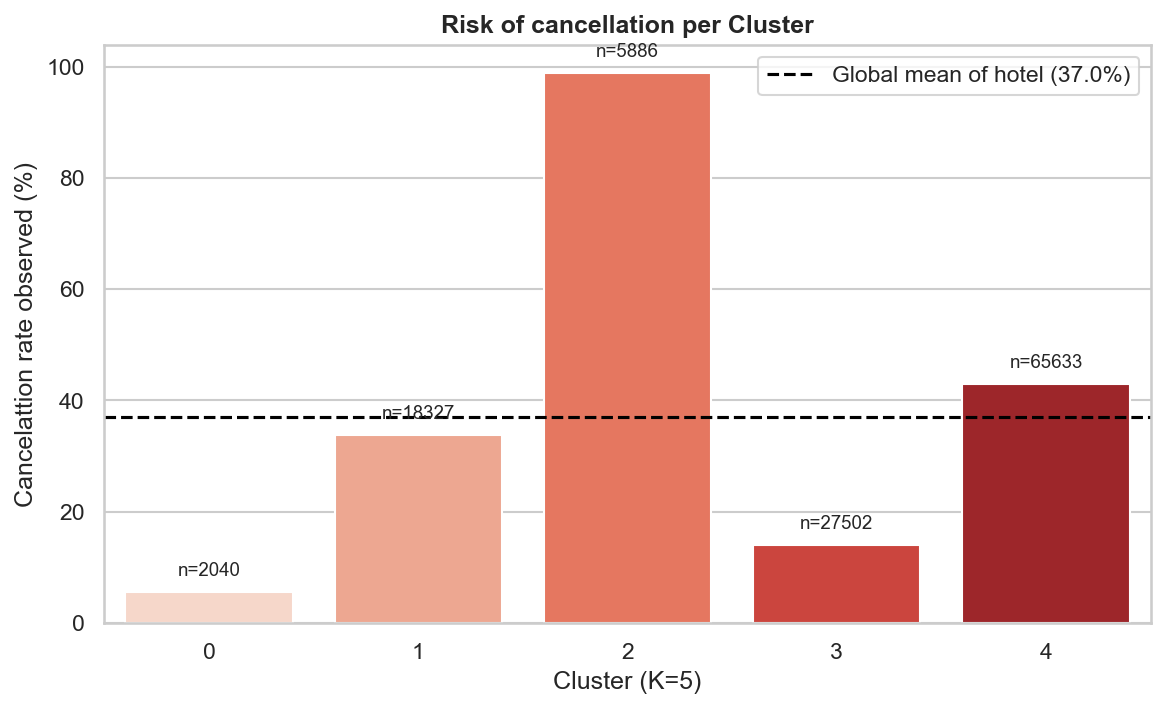
\includegraphics[width=0.80\textwidth]{figures/bar_cancellation_risk_by_cluster.png}
  \caption{Post-hoc cancellation rate per cluster (K-Means, $K=5$).
           The dashed line marks the global mean of 37.0\%.
           Cluster~2 ($n=5{,}886$) reaches 98.9\%; Cluster~3
           ($n=27{,}502$) attains only 14.0\%.
           Note that \texttt{is\_canceled} was \emph{not} used as a
           clustering input; these rates emerge purely from post-hoc
           profiling.}
  \label{fig:cancel_risk}
\end{figure}

\begin{figure}[H]
  \centering
  \begin{subfigure}[b]{0.48\textwidth}
    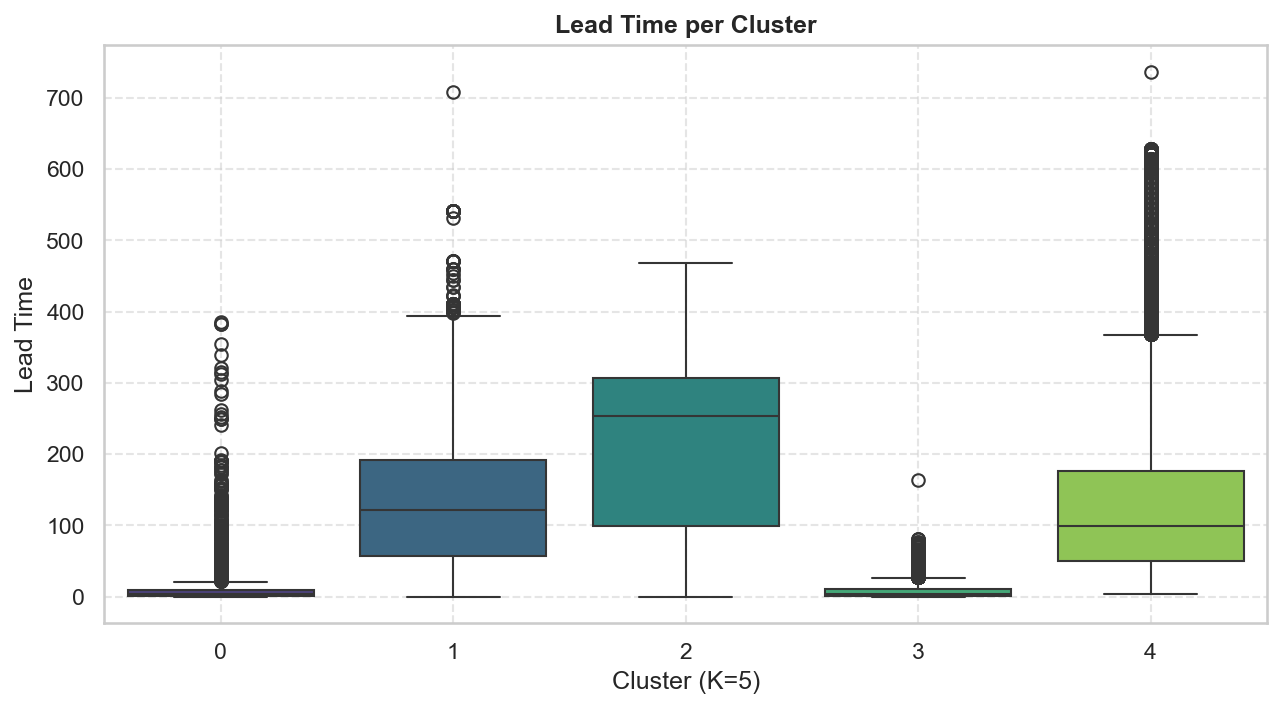
\includegraphics[width=\textwidth]{figures/boxplot_lead_time_by_cluster.png}
    \caption{Lead time distribution}
    \label{fig:lead_time}
  \end{subfigure}
  \hfill
  \begin{subfigure}[b]{0.48\textwidth}
    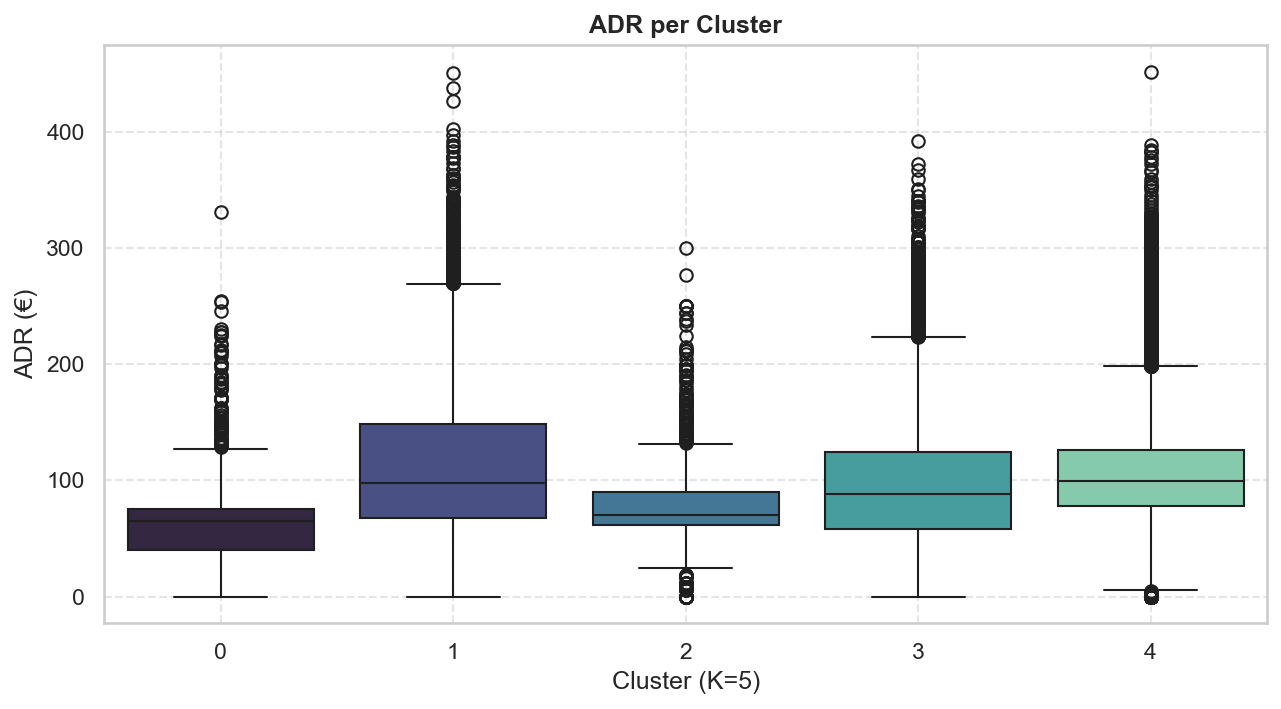
\includegraphics[width=\textwidth]{figures/boxplot_adr_by_cluster.png}
    \caption{ADR distribution (post-hoc)}
    \label{fig:adr}
  \end{subfigure}
  \caption{Lead time (clustering input) and ADR (post-hoc) box plots by
           cluster. Cluster~2 exhibits the longest lead times (median
           $\approx 250$ days) and below-average ADR ($\approx$\EUR{}72),
           consistent with low-cost speculative advance bookings.
           Cluster~3's near-zero lead time reflects last-minute direct
           bookings. ADR is only used for post-hoc profiling.}
  \label{fig:boxes}
\end{figure}

\begin{figure}[H]
  \centering
  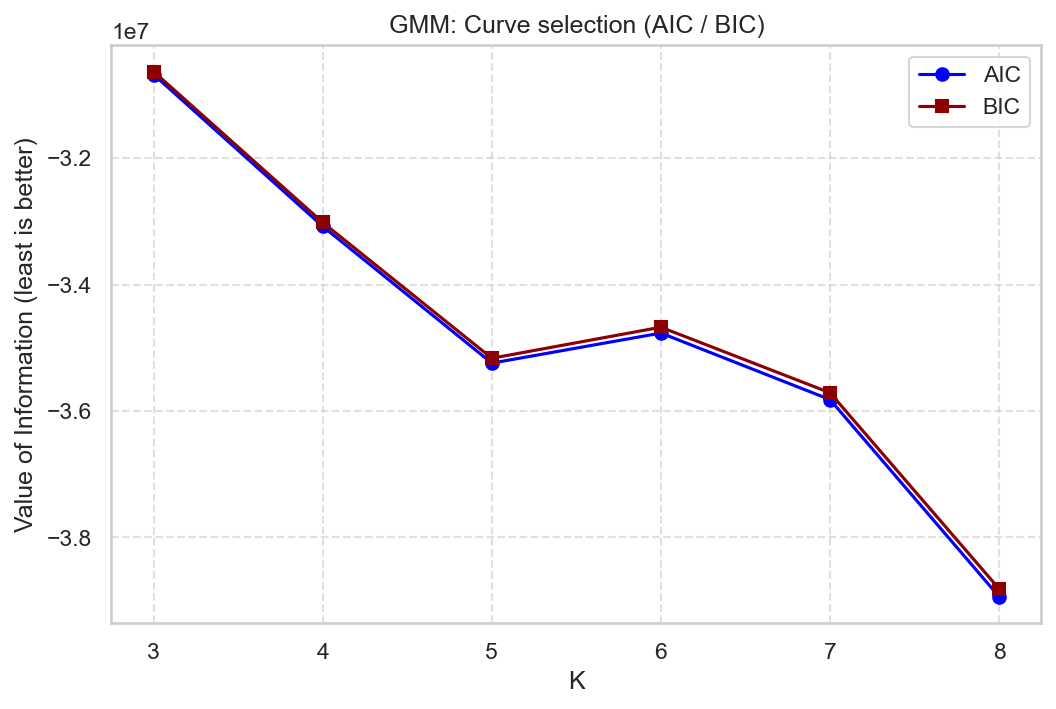
\includegraphics[width=0.75\textwidth]{figures/gmm_aic_bic_diagnostics.png}
  \caption{GMM model-selection curves (AIC and BIC) for
           $K \in \{3,\ldots,8\}$. Both criteria decrease monotonically
           without a clear elbow, indicating the data supports more
           components than the practical range tested.
           $K=5$ is adopted for consistency with K-Means; a larger $K$
           may be justified if interpretability of more granular components
           is a priority.}
  \label{fig:gmm_aic_bic}
\end{figure}

\begin{figure}[H]
  \centering
  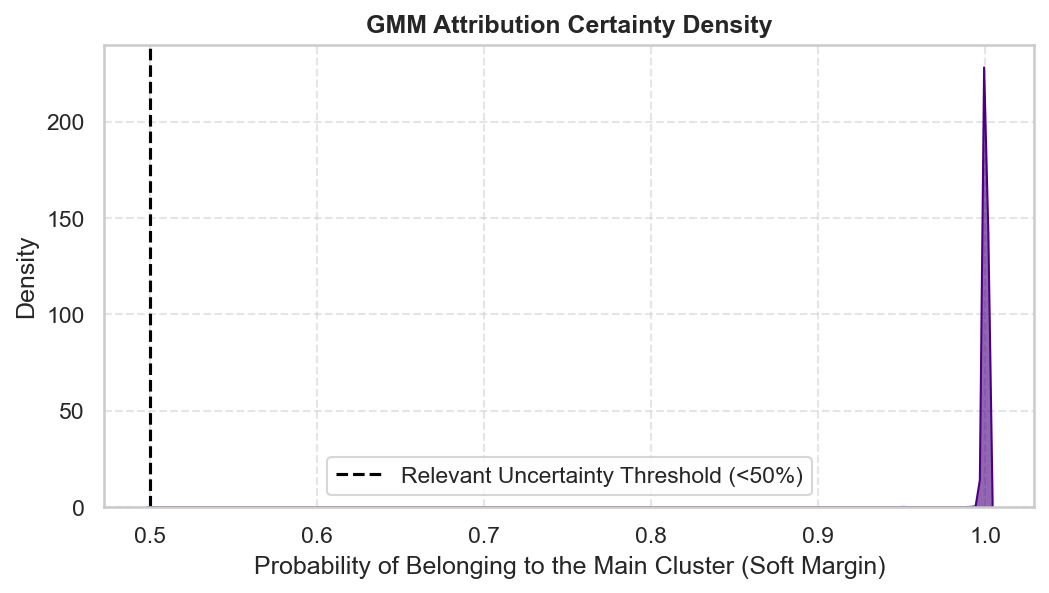
\includegraphics[width=0.75\textwidth]{figures/gmm_classification_certainty.png}
  \caption{GMM assignment certainty density. The distribution is highly
           concentrated near $p=1.0$, indicating that despite the soft
           probabilistic model, the great majority of bookings are
           unambiguously assigned to a single component.
           This supports the near-hard cluster structure found by K-Means.}
  \label{fig:gmm_certainty}
\end{figure}

\begin{figure}[H]
  \centering
  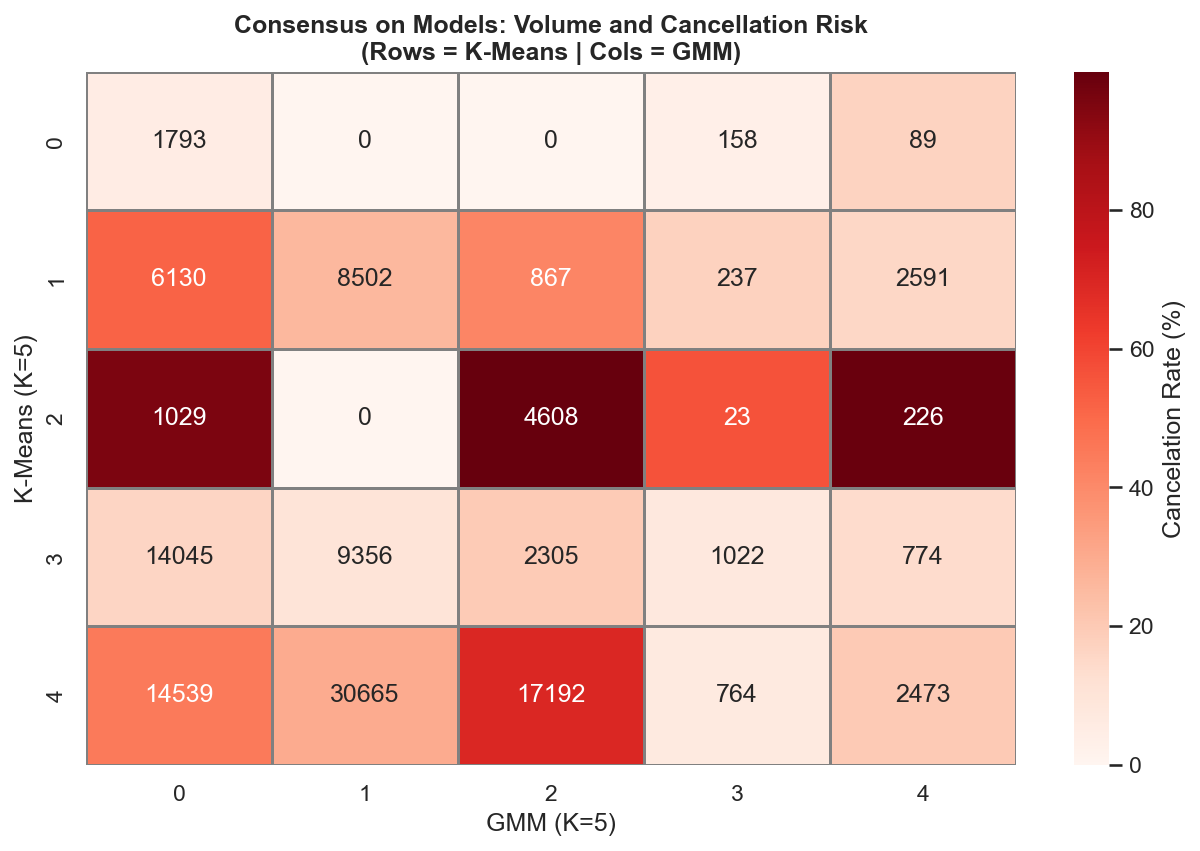
\includegraphics[width=0.85\textwidth]{figures/heatmap_consensus_models.png}
  \caption{Consensus matrix between K-Means and GMM ($K=5$).
           Rows are K-Means clusters; columns are GMM components; cell
           values are booking counts; colour encodes post-hoc cancellation
           rate. K-Means Cluster~2 (98.9\% cancellation) maps almost
           entirely to GMM Cluster~2 (dark red diagonal cell: 4,608 bookings),
           confirming that the critical high-risk segment is robustly
           identified across both modelling families.}
  \label{fig:consensus}
\end{figure}

\begin{figure}[H]
  \centering
  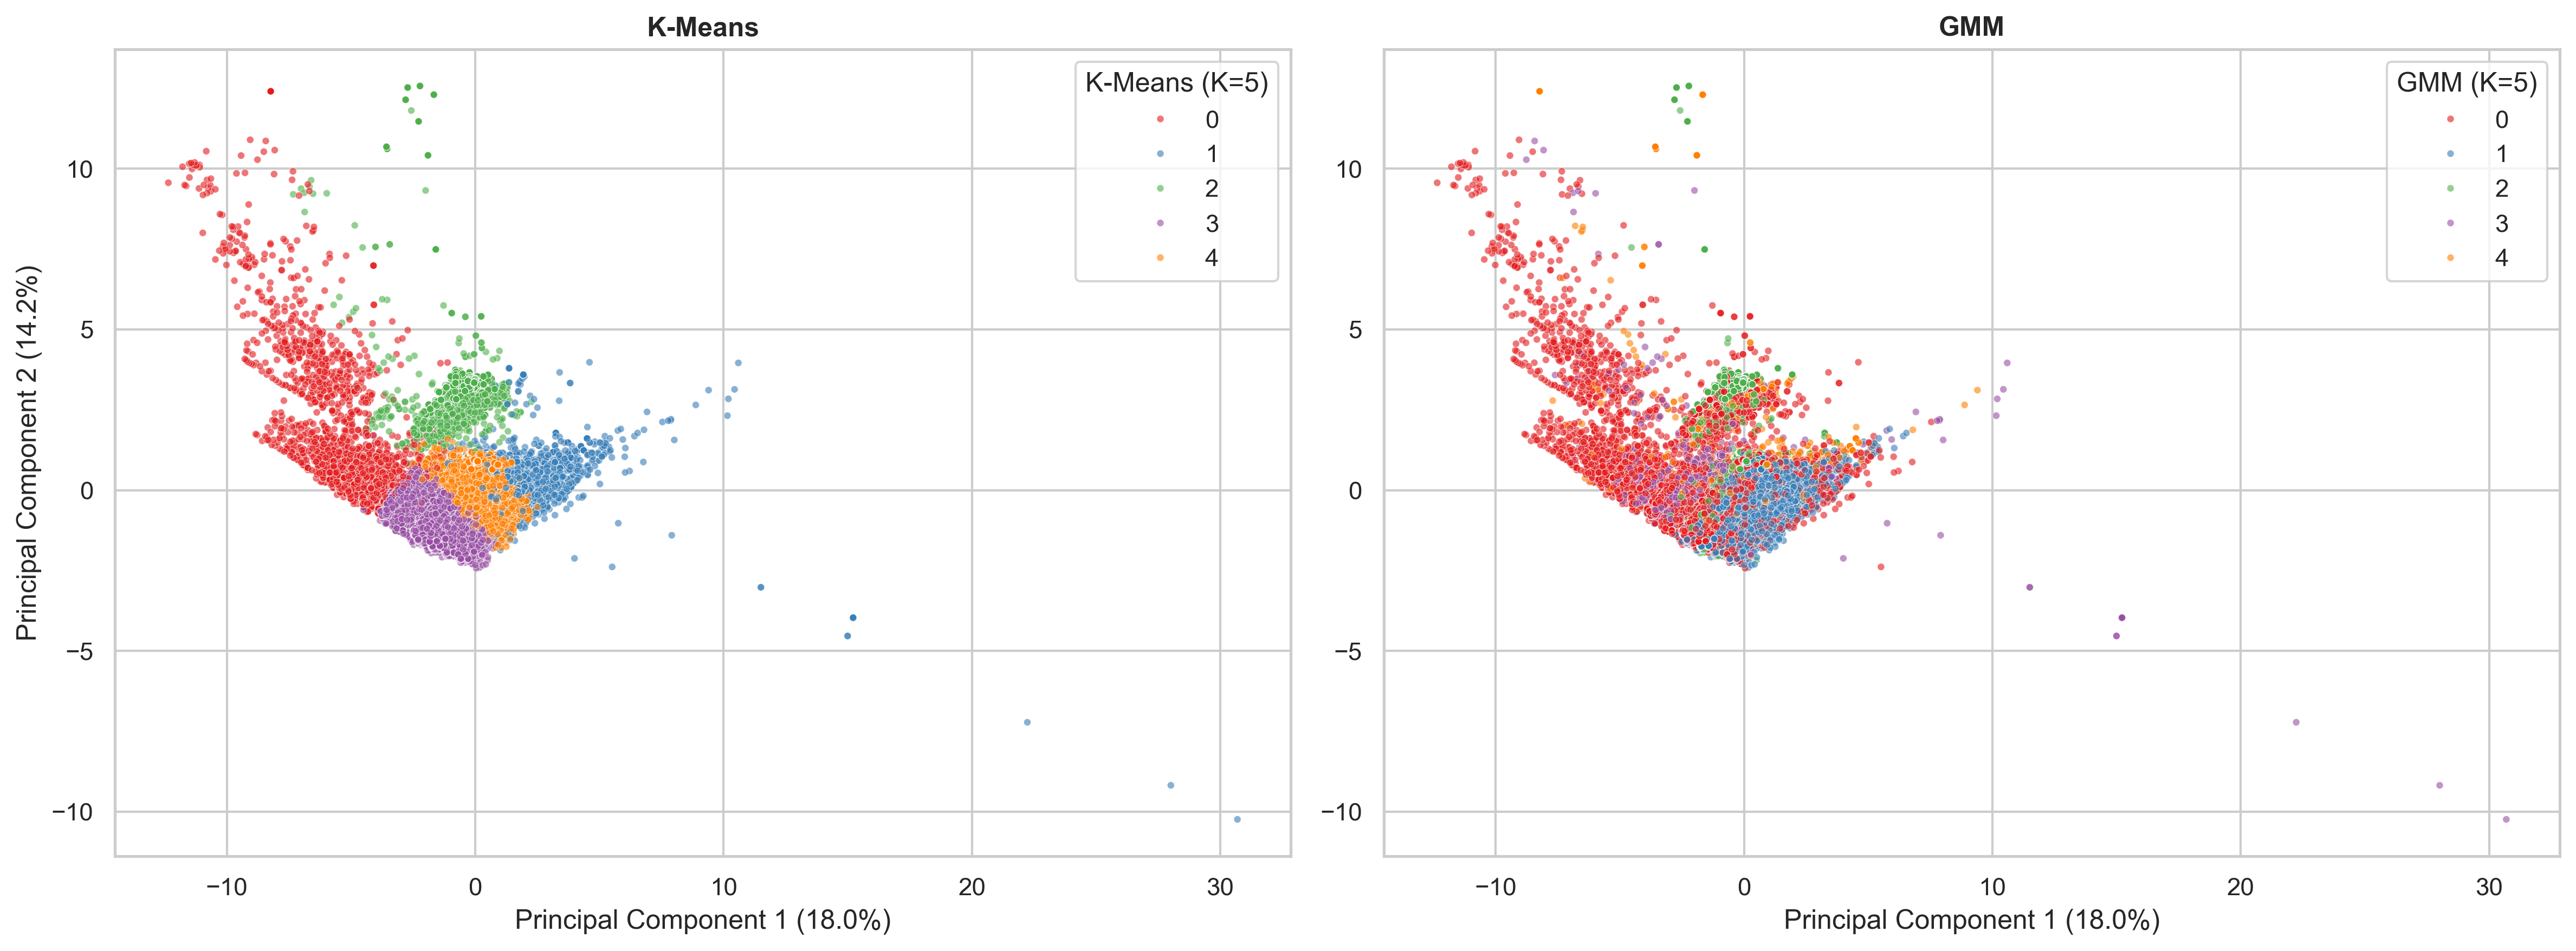
\includegraphics[width=\textwidth]{figures/pca_comparison_kmeans_vs_gmm.png}
  \caption{PCA projection (components 1 and 2, explaining 18.0\% and
           14.2\% of variance respectively) of K-Means vs GMM assignments
           at $K=5$. Both methods produce broadly similar spatial
           partitions. Cluster~2 (K-Means: green; GMM: green) occupies
           the upper-left region, corresponding to high lead time and
           high prior cancellation score in the PCA embedding.
           Note that PCA is used here for visualisation only; clustering
           was performed in the full 55-dimensional R-EUCLID space.}
  \label{fig:pca}
\end{figure}

\end{document}
